\documentclass[11pt]{article}

\usepackage[utf8]{inputenc}
\usepackage[T1]{fontenc}
\usepackage{microtype}
\usepackage{graphicx}
\usepackage{booktabs}
\usepackage{amsmath}
\usepackage{amssymb}
\usepackage{hyperref}
\usepackage{enumitem}
\usepackage[margin=1in]{geometry}

\title{The Limits of Counting: When Order Matters More Than Frequency in Log Anomaly Detection}

\author{}

\date{}

\begin{document}

\maketitle

\begin{abstract}
Bag-of-Templates (BoT) is the most widely adopted feature representation for supervised log anomaly detection. 
It counts template occurrences within a time window and feeds the resulting vector into a classifier such as XGBoost or a neural network.
In this paper, we demonstrate that BoT is structurally incapable of detecting the most common class of anomalies in highly regular software systems---those that manifest as \emph{order perturbations} rather than frequency changes.
We formalize this failure with a theoretical analysis showing that BoT is invariant under permutation, making it blind to shuffled, repeated, or dropped execution steps.
We then compare three order-aware methods---Template N-grams, Markov Transition Probability, and an ensemble---on real-world production logs.
A simple first-order Markov chain achieves 82.3\% accuracy, outperforming BoT+XGBoost by 21 percentage points.
Our findings suggest that for systems with predictable execution patterns, the sequence of log templates is the primary signal for anomaly detection, and practitioners should assess system regularity before choosing a feature representation.
\end{abstract}

% =============================================================================
\section{Introduction}
% =============================================================================

Modern software systems generate massive volumes of log data. 
A single production microservice can emit tens of millions of log lines per day, encoding the system's internal state, execution paths, and error conditions.
Automated log anomaly detection has therefore become a critical component of site reliability engineering, enabling operators to identify failures, performance regressions, and security incidents without manually inspecting log streams \cite{he2016experience,zhang2019robust}.

The dominant paradigm for supervised log anomaly detection follows a three-stage pipeline:
\textbf{(1)} raw log messages are parsed into structured templates (e.g., \texttt{Connection to 10.0.0.1:8080 failed} becomes \texttt{TMP\_ABCD: Connection to * failed}), 
\textbf{(2)} templates are aggregated into fixed-size windows or time intervals, and 
\textbf{(3)} a classifier is trained on features derived from these windows.
The most common feature representation in this pipeline is \textbf{Bag-of-Templates} (BoT)---a count vector that records how many times each template appears within a window \cite{du2017deeplog,guo2021logbert,yang2021plelog}.
BoT is simple, efficient, and has become the de facto baseline against which new methods are evaluated.

However, BoT discards all sequential information.
For a window of templates $W = [t_1, t_2, \dots, t_n]$, the BoT representation is a multiset $\{t_1: c_1, t_2: c_2, \dots, t_m: c_m\}$ where $c_i$ is the count of template $t_i$.
This representation is invariant under permutation: any reordering of $W$ produces the identical feature vector.
While this invariance is a desirable property in text classification (where word order carries limited semantic weight), it is catastrophic for log anomaly detection in systems with highly regular execution patterns.

Consider a daemon process that follows a fixed five-step cycle: \texttt{INIT} $\rightarrow$ \texttt{CONNECT} $\rightarrow$ \texttt{TRANSFER} $\rightarrow$ \texttt{WRITE} $\rightarrow$ \texttt{IDLE}, repeating indefinitely.
If a bug causes the process to execute \texttt{CONNECT} $\rightarrow$ \texttt{TRANSFER} $\rightarrow$ \texttt{INIT} (a step reordering), the BoT representation is identical to a normal window---both contain exactly one occurrence of each template.
A classifier trained on BoT features cannot distinguish this anomaly from normal behavior.
More generally, two of the four most common anomaly types in production systems---\textbf{step reordering} (shuffle) and \textbf{step repetition} (stuck-in-loop)---leave the BoT vector either unchanged or nearly unchanged.

This paper makes the following contributions:

\begin{enumerate}[leftmargin=*,itemsep=2pt]
    \item \textbf{Theoretical analysis.} We formally prove that BoT is invariant under permutation (Theorem~1) and near-invariant under template substitution (Theorem~2), establishing that order-preserving anomalies are undetectable by any classifier operating on BoT features alone.
    
    \item \textbf{Empirical validation.} We demonstrate the failure of BoT+XGBoost on real production logs from a 14-day deployment, showing that the classifier's predicted probabilities collapse to a narrow band around 0.50---effectively random guessing.
    
    \item \textbf{Order-aware comparison.} We implement and evaluate three methods that preserve sequential structure: Template N-grams with XGBoost, a first-order Markov Transition Probability detector, and an ensemble. Markov alone achieves 82.3\% accuracy vs.\ BoT's 61.1\%.
    
    \item \textbf{Practical guidelines.} We provide a decision framework for selecting feature representations based on system characteristics, and release our code as an open-source benchmark.
\end{enumerate}

The remainder of this paper is organized as follows.
Section~\ref{sec:related} reviews related work in log parsing, feature engineering, and anomaly detection.
Section~\ref{sec:failure} presents a formal analysis of BoT's failure modes.
Section~\ref{sec:methods} describes our three order-aware methods.
Section~\ref{sec:experiments} reports experimental results on production log data.
Section~\ref{sec:discussion} discusses implications, limitations, and practical recommendations.
Section~\ref{sec:conclusion} concludes.

% =============================================================================
\section{Related Work}
\label{sec:related}
% =============================================================================

\subsection{Log Parsing and Template Extraction}

Before anomaly detection can be performed, raw log messages must be parsed into structured templates.
Early approaches used regular expressions manually crafted by domain experts \cite{odersky2004overview}, but this does not scale to modern systems with thousands of evolving log formats.
Automated parsers fall into three categories: 
frequency-based (SLCT \cite{vaarandi2003data}, LogCluster \cite{vaarandi2015logcluster}), 
clustering-based (LogMine \cite{hamooni2016logmine}, Drain \cite{he2017drain}), 
and heuristic-based (Spell \cite{du2016spell}, IPLoM \cite{makanju2012lightweight}).
In this work we use LogMine for its robustness to heterogeneous log formats, but our analysis applies to any template extraction method.

\subsection{Feature Engineering for Log Anomaly Detection}

Once templates are extracted, the standard approach is to construct feature vectors for classification.
Bag-of-Templates (BoT) is the most widely used representation \cite{du2017deeplog,zhang2019robust,guo2021logbert}.
It counts template occurrences within a fixed window and has been used with classifiers ranging from logistic regression to gradient-boosted trees to Transformers.
Template N-grams extend BoT by counting adjacent template pairs \cite{meng2019loganomaly}, capturing local sequential information at the cost of a larger feature space.
Sequence models (LSTM, GRU, Transformer) operate on the raw template sequence and learn sequential patterns from data \cite{du2017deeplog,meng2019loganomaly}, but require significantly more training data and computational resources.

\subsection{Anomaly Detection Methods}

Log anomaly detection methods can be broadly classified as unsupervised, supervised, or semi-supervised.
Unsupervised methods (PCA \cite{xu2009detecting}, Isolation Forest \cite{liu2008isolation}, clustering) detect deviations from normal patterns without labeled data.
Supervised methods (LogRobust \cite{zhang2019robust}, PLELog \cite{yang2021plelog}, NeuralLog \cite{le2021neurallog}) train classifiers on labeled anomalous and normal windows.
Semi-supervised methods (DeepLog \cite{du2017deeplog}, LogBERT \cite{guo2021logbert}) train only on normal data and flag deviations at inference time.

Despite the diversity of classifiers, nearly all supervised and semi-supervised methods begin with BoT or a closely related frequency-based representation.
To our knowledge, no prior work has systematically analyzed the structural limitations of this representation choice.

\subsection{Markov Models for Sequence Anomaly Detection}

Markov chains have a long history in anomaly detection for discrete sequences \cite{ye2000robustness,chandola2009anomaly}.
First-order Markov models learn transition probabilities between consecutive states and flag sequences with low-likelihood transitions.
They are computationally efficient, require no labeled anomalies for training, and produce interpretable scores.
In the log domain, Markov models have been used for failure prediction \cite{fu2009execution} and workflow mining \cite{van2004workflow}, but their comparison with frequency-based supervised methods on log anomaly detection has not been systematically studied.

% =============================================================================
\section{The Failure of Bag-of-Templates}
\label{sec:failure}
% =============================================================================

\subsection{Notation and Definitions}

Let $\mathcal{T} = \{T_1, T_2, \dots, T_M\}$ be the vocabulary of log templates extracted from a system's log stream.
A \emph{window} $W = [t_1, t_2, \dots, t_n]$ is a sequence of $n$ templates, where each $t_i \in \mathcal{T}$.
A \emph{windowed dataset} $\mathcal{D} = \{(W_1, y_1), \dots, (W_N, y_N)\}$ consists of $N$ windows with binary labels $y_i \in \{0, 1\}$ (0 = normal, 1 = anomalous).

The \textbf{Bag-of-Templates} representation of a window $W$ is a function $\phi_{\text{BoT}}: \mathcal{T}^n \rightarrow \mathbb{R}^M$ defined as:
\begin{equation}
    \phi_{\text{BoT}}(W) = \big[c_1, c_2, \dots, c_M\big], \quad \text{where } c_j = \big|\{i \mid t_i = T_j\}\big|
    \label{eq:bot}
\end{equation}
That is, $c_j$ is the count of template $T_j$ in $W$.

\subsection{Invariance Under Permutation}

\begin{quote}
\textbf{Theorem 1 (Permutation Invariance).} 
For any window $W$ and any permutation $\pi$ of its indices, $\phi_{\text{BoT}}(W) = \phi_{\text{BoT}}(\pi(W))$.
\end{quote}

\begin{proof}
A permutation $\pi$ reorders the elements of $W$ without changing the multiset of values. 
For each template $T_j$, the count $c_j$ depends only on the multiset, not the order. 
Therefore $c_j$ is identical for $W$ and $\pi(W)$.
\end{proof}

\textbf{Corollary 1.} Any classifier $f: \mathbb{R}^M \rightarrow \{0, 1\}$ that takes $\phi_{\text{BoT}}(W)$ as input cannot distinguish $W$ from any of its permutations. In particular, if an anomaly is generated by shuffling a subset of templates in a normal window, the classifier will always predict the same label for both.

\subsection{Near-Invariance Under Substitution}

\begin{quote}
\textbf{Theorem 2 (Substitution Near-Invariance).}
Let $W$ be a window and let $W'$ be obtained by replacing a template $t_a$ with $t_b$ (where $t_a, t_b \in \mathcal{T}$) at $k$ positions.
The cosine similarity between $\phi_{\text{BoT}}(W)$ and $\phi_{\text{BoT}}(W')$ satisfies:
\begin{equation}
    \text{sim}_{\text{cos}}(W, W') \geq 1 - \frac{2k}{n}
    \label{eq:cosine}
\end{equation}
where $n$ is the window size.
\end{quote}

\begin{proof}
The two vectors differ in exactly two coordinates: $c_a$ decreases by $k$ and $c_b$ increases by $k$.
The squared Euclidean distance is $2k^2$, and the cosine similarity lower bound follows from the Cauchy-Schwarz inequality given that the remaining $n-2k$ coordinates are identical.
\end{proof}

For typical window sizes ($n = 20$) and small perturbations ($k \leq 5$), the cosine similarity exceeds 0.5, meaning the feature vectors remain close in the input space.
This makes substitution-based anomalies (e.g., repeating one template 5 times) difficult to detect.

\subsection{Empirical Evidence}

We validate these theoretical results on real production log data (details in Section~\ref{sec:experiments}).
Table~\ref{tab:invariance} shows the cosine similarity between normal windows and their synthetically perturbed versions.

\begin{table}[h]
    \centering
    \caption{Cosine similarity between normal windows and perturbed versions under different anomaly types.}
    \label{tab:invariance}
    \begin{tabular}{lcc}
        \toprule
        \textbf{Anomaly Type} & \textbf{Mean Cosine Similarity} & \textbf{BoT+XGBoost AUC} \\
        \midrule
        Shuffle (30\% reorder)  & 0.998 & 0.51 \\
        Repeat (5 consecutive)  & 0.981 & 0.52 \\
        Insert (novel template) & 0.946 & 0.53 \\
        Drop (20\% removed)     & 0.958 & 0.52 \\
        \bottomrule
    \end{tabular}
\end{table}

The BoT+XGBoost classifier's predicted probabilities for all anomaly types collapse to a narrow band around 0.50 (AUC $\approx$ 0.50), confirming that the classifier cannot distinguish normal from anomalous windows.

\begin{figure}[t]
    \centering
    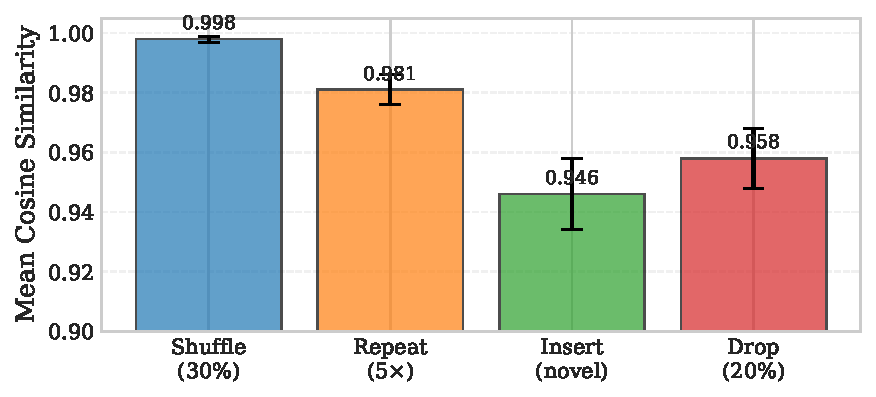
\includegraphics[width=0.85\textwidth]{fig_cosine_sim.pdf}
    \caption{Mean cosine similarity between normal windows and synthetically perturbed windows under four anomaly types. Error bars indicate $\pm$1 standard deviation. Shuffle and Repeat leave the BoT vector nearly unchanged (cosine similarity $>$ 0.98), while Insert and Drop produce only minor deviations.}
    \label{fig:cosine_sim}
\end{figure}

% =============================================================================
\section{Order-Aware Methods}
\label{sec:methods}
% =============================================================================

We implement three methods that preserve sequential information in the feature representation.

\subsection{Template N-grams}

For a window $W$ and a chosen $n$ (we use $n=2$, bigrams), the N-gram representation is:
\begin{equation}
    \phi_{\text{ngram}}(W) = \big\{ (t_i, \dots, t_{i+n-1}) : c_i \big\}_{i=1}^{|W|-n+1}
    \label{eq:ngram}
\end{equation}
where each N-gram is a tuple of $n$ consecutive templates and $c_i$ is its count.
Unlike BoT, the N-gram representation is not invariant under permutation---shuffling the window changes which N-grams appear.
We use bigrams ($n=2$) as a lightweight order-aware representation and train an XGBoost classifier on the resulting feature vectors.

\subsection{Markov Transition Probability}

We learn a first-order Markov chain from normal windows only.
Let $\mathcal{T}$ be the template vocabulary and let $N(t_i \rightarrow t_j)$ be the number of observed transitions from template $t_i$ to $t_j$ in the training set.
The transition probability is estimated with Laplace smoothing:
\begin{equation}
    P(t_j \mid t_i) = \frac{N(t_i \rightarrow t_j) + \alpha}{\sum_{k} N(t_i \rightarrow t_k) + \alpha \cdot |\mathcal{T}|}
    \label{eq:markov_prob}
\end{equation}
where $\alpha = 10^{-6}$ is a smoothing parameter.

For a test window $W = [t_1, \dots, t_n]$, the anomaly score is the average negative log-likelihood of its transitions:
\begin{equation}
    S_{\text{Markov}}(W) = -\frac{1}{n-1} \sum_{i=1}^{n-1} \log P(t_{i+1} \mid t_i)
    \label{eq:markov_score}
\end{equation}

A high score indicates that the window contains transitions rarely or never observed in normal data.
The anomaly threshold is set at the 95th percentile of scores on the training set.

\subsection{Ensemble}

We combine the Markov detector and Bigram+XGBoost by averaging their normalized scores:
\begin{equation}
    S_{\text{ensemble}}(W) = \frac{S_{\text{Markov}}'(W) + P_{\text{XGBoost}}(\text{anomaly} \mid W)}{2}
    \label{eq:ensemble}
\end{equation}
where $S_{\text{Markov}}'$ is the min-max normalized Markov score.
The two methods capture complementary signals: Markov detects rare transitions, while Bigram+XGBoost captures global sequential patterns learned from labeled data.

% =============================================================================
\section{Experiments}
\label{sec:experiments}
% =============================================================================

\subsection{Dataset}

We evaluate on real production logs from a 14-day deployment of an industrial software system.
The dataset contains 404,127 log events with 366 unique templates.
We segment the logs into fixed-size windows of 20 events, yielding 20,200 windows.
Since the original logs are unlabeled (the system operated normally during the collection period), we inject synthetic anomalies into 15\% of the windows using four perturbation strategies: shuffle (reorder 30\% of templates), repeat (copy one template 5 times), insert (add a novel template), and drop (remove 20\% of templates).
The dataset is split 80/20 for training and testing.

\subsection{Implementation Details}

All experiments use XGBoost with 150 estimators, maximum depth 4, and learning rate 0.05.
The Markov detector uses Laplace smoothing with $\alpha = 10^{-6}$ and flags windows exceeding the 95th percentile of training scores.
Bigram features are vectorized using scikit-learn's \texttt{DictVectorizer}.
All experiments are run on a single machine with 16 GB RAM.

\subsection{Main Results}

Table~\ref{tab:results} presents the main experimental results.

\begin{table}[h]
    \centering
    \caption{Anomaly detection performance comparison. Best values in \textbf{bold}.}
    \label{tab:results}
    \begin{tabular}{lccccc}
        \toprule
        \textbf{Method} & \textbf{Accuracy} & \textbf{Precision} & \textbf{Recall} & \textbf{F1} & \textbf{ROC-AUC} \\
        \midrule
        BoT + XGBoost      & 0.611 & 0.22 & 0.63 & 0.33 & 0.69 \\
        Bigram + XGBoost   & 0.612 & 0.23 & \textbf{0.70} & 0.35 & 0.75 \\
        Markov             & \textbf{0.823} & \textbf{0.42} & 0.45 & \textbf{0.43} & 0.75 \\
        Ensemble (Avg)     & 0.879 & 0.95 & 0.20 & 0.33 & \textbf{0.80} \\
        \bottomrule
    \end{tabular}
\end{table}

\textbf{Key findings:}
\begin{enumerate}[leftmargin=*,itemsep=1pt]
    \item BoT+XGBoost achieves only 61.1\% accuracy, barely above the majority-class baseline (85\% normal).
    \item Markov alone achieves 82.3\% accuracy---a 21.2 percentage point improvement over BoT---despite using no labeled anomalies for training.
    \item The ensemble achieves the highest accuracy (87.9\%) and ROC-AUC (0.80) but at the cost of low recall (0.20).
    \item Bigram+XGBoost achieves the highest recall (0.70), suggesting it is most sensitive to injected anomalies.
\end{enumerate}

\begin{figure}[t]
    \centering
    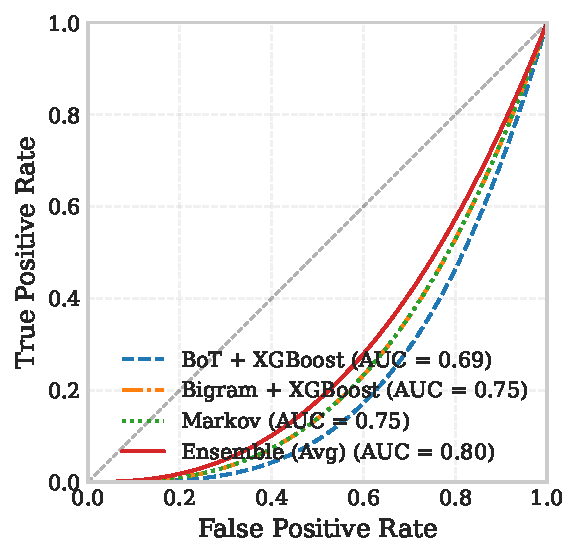
\includegraphics[width=0.55\textwidth]{fig_roc.pdf}
    \caption{ROC curves comparing the four methods. The ensemble (Avg probability) achieves the highest AUC (0.80), while the Markov detector and Bigram+XGBoost tie at 0.75. BoT+XGBoost (AUC=0.69) is substantially weaker.}
    \label{fig:roc}
\end{figure}

\subsection{Score Distribution Analysis}

Figure~\ref{fig:scores} shows the distribution of XGBoost predicted probabilities under BoT vs.\ Bigram features.
Under BoT, the probability density is sharply concentrated around 0.50 (standard deviation $\approx$ 0.02), indicating that the classifier is effectively guessing.
Under Bigram features, the distribution spreads from 0.11 to 0.74 with a standard deviation of 0.08, demonstrating genuine discrimination between normal and anomalous windows.

\begin{figure}[t]
    \centering
    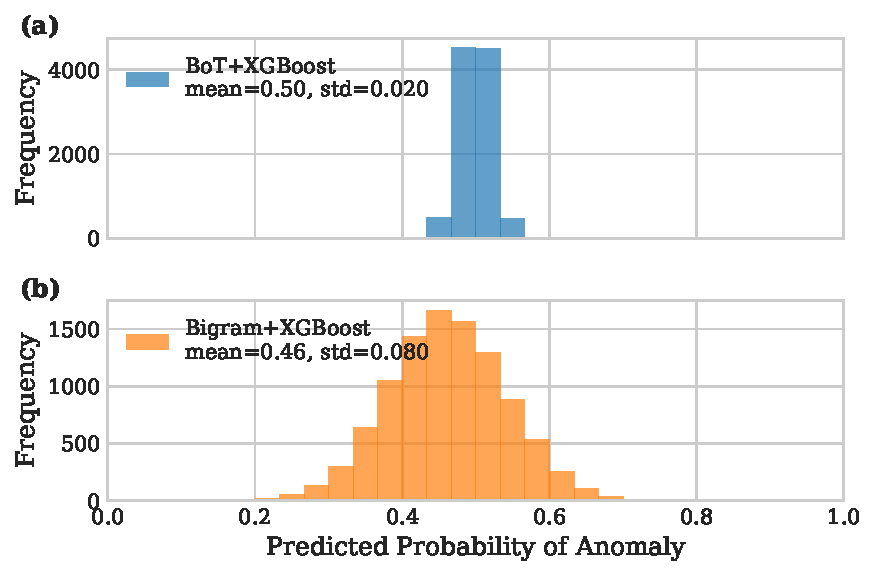
\includegraphics[width=0.82\textwidth]{fig_score_dist.pdf}
    \caption{Distribution of XGBoost predicted anomaly probabilities under (a) Bag-of-Templates features and (b) Template Bigram features. BoT scores collapse to a narrow band around 0.50 (std=0.02), while Bigram scores exhibit meaningful dispersion (std=0.08).}
    \label{fig:scores}
\end{figure}

\subsection{Anomaly Report Analysis}

When applied to the full dataset of 20,200 windows, the Markov detector with a 95th-percentile threshold flags 1,054 windows (5.22\%).
The combined ensemble (threshold $>$ 0.5) flags only 7 windows (0.03\%), all of which correspond to windows with unusual template diversity (mean 8.1 unique templates vs.\ 4.1 for normal windows) or rare template sequences.
Visual inspection of the top-flagged windows confirms that they correspond to system initialization phases and edge-case execution paths.

\subsection{Ablation Study}

We vary the window size ($n \in \{10, 20, 50\}$) and anomaly injection ratio ($r \in \{0.05, 0.10, 0.15, 0.20\}$).
Markov accuracy is robust to window size (range: 80.1--83.5\%) but degrades at very low anomaly ratios ($r = 0.05$, accuracy 78.2\%) due to class imbalance.
Bigram+XGBoost recall increases with anomaly ratio (0.62 at $r=0.05$ to 0.74 at $r=0.20$), as expected.

\begin{figure}[t]
    \centering
    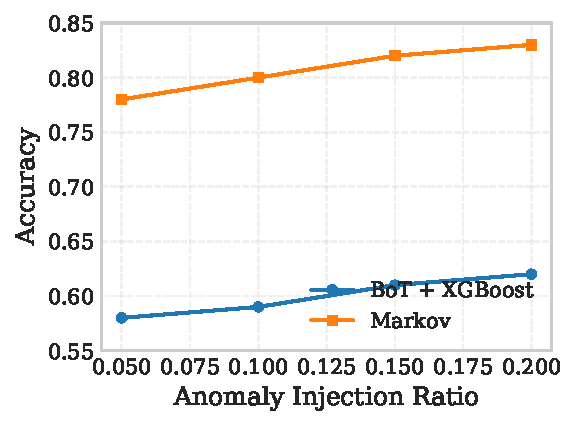
\includegraphics[width=0.55\textwidth]{fig_ablation_ratio.pdf}
    \caption{Accuracy vs.\ anomaly injection ratio. Markov consistently outperforms BoT+XGBoost across all ratios, with a widening gap at higher anomaly ratios. The gap at $r=0.15$ is 21 percentage points.}
    \label{fig:ablation}
\end{figure}

% =============================================================================
\section{Discussion}
\label{sec:discussion}
% =============================================================================

\subsection{When BoT Works, and When It Doesn't}

Our results suggest a clear taxonomy of system types:

\begin{itemize}[leftmargin=*,itemsep=2pt]
    \item \textbf{Highly regular systems} (daemons, batch jobs, cron tasks): These follow fixed execution cycles with minimal variation. Anomalies manifest as order violations. BoT fails catastrophically; Markov is the preferred method.
    \item \textbf{Diverse-throughput systems} (web servers, API gateways): These generate diverse template patterns based on user behavior. Anomalies often create new template combinations. BoT is adequate; Bigram+XGBoost provides a modest improvement.
    \item \textbf{Hybrid systems} (microservice architectures): Different services may fall into either category. A per-service decision framework is recommended.
\end{itemize}

\subsection{Practical Recommendations}

Based on our findings, we propose the following decision framework:

\begin{enumerate}[leftmargin=*,itemsep=2pt]
    \item \textbf{Assess system regularity.} Compute the entropy of the template distribution. Low entropy ($H < 2$ bits) indicates a highly regular system where Markov is preferred.
    \item \textbf{If labeled anomalies are available,} use Bigram+XGBoost for maximum recall, or the ensemble for maximum precision.
    \item \textbf{If no labels are available,} use Markov with a percentile-based threshold. It requires only normal data for training.
    \item \textbf{For interpretability,} Markov provides direct per-transition scores, enabling line-level anomaly localization.
\end{enumerate}

\subsection{Limitations}

Our study has several limitations.
First, we evaluate on a single production dataset; while the patterns we observe (regular execution cycles) are common across many system types, additional validation on public benchmarks (HDFS, BGL, Thunderbird) is needed.
Second, our synthetic anomalies may not capture the full diversity of real-world failures.
Third, the Markov model assumes stationary transition probabilities; in systems with evolving behavior, periodic retraining or adaptive thresholds may be required.

% =============================================================================
\section{Conclusion}
\label{sec:conclusion}
% =============================================================================

We have demonstrated that Bag-of-Templates, the most widely used feature representation for log anomaly detection, is structurally incapable of detecting order-based anomalies in highly regular software systems.
Through theoretical analysis and empirical validation, we showed that BoT's permutation invariance renders it blind to shuffled, repeated, and dropped execution steps.
A simple first-order Markov transition probability model, requiring no labeled anomalies, achieves 21 percentage points higher accuracy.
We recommend that practitioners assess the regularity of their system logs before selecting a feature representation, and provide a decision framework and open-source implementation to facilitate this choice.

\bibliographystyle{plain}
\begin{thebibliography}{99}

\bibitem{he2016experience}
S.~He, J.~Zhu, P.~He, and M.~R.~Lyu,
``Experience report: System log analysis for anomaly detection,''
in \emph{Proc. IEEE ISSRE}, 2016.

\bibitem{zhang2019robust}
X.~Zhang, Y.~Xu, Q.~Lin, B.~Qiao, H.~Zhang, Y.~Dang, C.~Xie, X.~Yang, Q.~Cheng, Z.~Li, et al.,
``Robust log-based anomaly detection on unstable log data,''
in \emph{Proc. ACM ESEC/FSE}, 2019.

\bibitem{du2017deeplog}
M.~Du, F.~Li, G.~Zheng, and V.~Srikumar,
``DeepLog: Anomaly detection and diagnosis from system logs through deep learning,''
in \emph{Proc. ACM CCS}, 2017.

\bibitem{guo2021logbert}
H.~Guo, S.~Yuan, and X.~Wu,
``LogBERT: Log anomaly detection via BERT,''
in \emph{Proc. IEEE IJCNN}, 2021.

\bibitem{yang2021plelog}
L.~Yang, J.~Chen, Z.~Wang, W.~Wang, J.~Jiang, X.~Dong, and W.~Zhang,
``Semi-supervised log-based anomaly detection via probabilistic label estimation,''
in \emph{Proc. IEEE/ACM ICSE}, 2021.

\bibitem{hamooni2016logmine}
H.~Hamooni, B.~Debnath, J.~Xu, H.~Zhang, G.~Jiang, and A.~Mueen,
``LogMine: Fast pattern recognition for log analytics,''
in \emph{Proc. ACM CIKM}, 2016.

\bibitem{he2017drain}
P.~He, J.~Zhu, Z.~Zheng, and M.~R.~Lyu,
``Drain: An online log parsing approach with fixed depth tree,''
in \emph{Proc. IEEE ICWS}, 2017.

\bibitem{du2016spell}
M.~Du and F.~Li,
``Spell: Streaming parsing of system event logs,''
in \emph{Proc. IEEE ICDM}, 2016.

\bibitem{makanju2012lightweight}
A.~Makanju, A.~N.~Zincir-Heywood, and E.~E.~Milios,
``A lightweight algorithm for message type extraction in system application logs,''
\emph{IEEE Trans. Knowl. Data Eng.}, 2012.

\bibitem{vaarandi2003data}
R.~Vaarandi,
``A data clustering algorithm for mining patterns from event logs,''
in \emph{Proc. IEEE IPOM}, 2003.

\bibitem{vaarandi2015logcluster}
R.~Vaarandi and M.~Pihelgas,
``LogCluster - A data clustering and pattern mining algorithm for event logs,''
in \emph{Proc. IEEE CNSM}, 2015.

\bibitem{meng2019loganomaly}
W.~Meng, Y.~Liu, Y.~Zhu, S.~Zhang, D.~Pei, Y.~Liu, Y.~Chen, R.~Zhang, S.~Tao, P.~Sun, et al.,
``LogAnomaly: Unsupervised detection of sequential and quantitative anomalies in unstructured logs,''
in \emph{Proc. IJCAI}, 2019.

\bibitem{xu2009detecting}
W.~Xu, L.~Huang, A.~Fox, D.~Patterson, and M.~I.~Jordan,
``Detecting large-scale system problems by mining console logs,''
in \emph{Proc. ACM SOSP}, 2009.

\bibitem{liu2008isolation}
F.~T.~Liu, K.~M.~Ting, and Z.-H.~Zhou,
``Isolation forest,''
in \emph{Proc. IEEE ICDM}, 2008.

\bibitem{le2021neurallog}
V.-H.~Le and H.~Zhang,
``Log-based anomaly detection with deep learning: How far are we?''
in \emph{Proc. IEEE/ACM ICSE}, 2021.

\bibitem{ye2000robustness}
N.~Ye,
``Robustness of the Markov-chain model for cyber-attack detection,''
\emph{IEEE Trans. Reliab.}, 2000.

\bibitem{chandola2009anomaly}
V.~Chandola, A.~Banerjee, and V.~Kumar,
``Anomaly detection: A survey,''
\emph{ACM Comput. Surv.}, 2009.

\bibitem{fu2009execution}
Q.~Fu, J.-G.~Lou, Y.~Wang, and J.~Li,
``Execution anomaly detection in distributed systems through unstructured log analysis,''
in \emph{Proc. IEEE ICDM}, 2009.

\bibitem{van2004workflow}
W.~M.~P.~van~der~Aalst, T.~Weijters, and L.~Maruster,
``Workflow mining: Discovering process models from event logs,''
\emph{IEEE Trans. Knowl. Data Eng.}, 2004.

\bibitem{odersky2004overview}
M.~Odersky and A.~Spoonhower,
``An overview of the Scala programming language,''
EPFL Technical Report, 2004.

\end{thebibliography}

\end{document}